\chapter{The Experiment}

\section{Setup}

\subsection{Hardware}

All the tests were conducted on a laptop with a commodity processor
(Intel\textregistered Core\texttrademark $\,i5$ at $2.40$GHz). In
order to enforce serial execution \footnote{We are talking about BLAS
  or LAPACK; as the high level algorithms used were serial.}, even
when low level libraries attempted multi-threading, we used the Linux
\emph{taskset} command. The laptop has $8$Gb of RAM, but only 512Mb
were used on each experiment (and only for dense matrix algorithms;
sparse ones used much less). \\

\subsection{Software}

The implementations used for the algorithms were basically Python
wrappers against native libraries. These packages were SciPy
\cite{scipy} and NetworkX \cite{networkx}. On the other hand, the
native libraries actually offering the algorithm implementations were:

\begin{itemize}
  \item LAPACK \cite{lapack}, which provides (among many other things)
    the MRRR implementation. LAPACK is actually the industrial
    standard for dense matrix computations. LAPACK is implemented in
    Fortran90 \footnote{At least the opensource version we used, as
      there are other commercial implementations as well.}.

  \item ARPACK \cite{arpack}, which provides the variant of the
    Lanczos algorithm that we tested (IRLM). It also relies on LAPACK
    as a lower layer. ARPACK is implemented in Fortran77.

  \item Scipy \cite{scipy}, which delivers the implementation of
    LOBPCG that we tested. While Scipy may also use LAPACK for several
    operations, is interesting that LOBPCG is the only algorithm that
    is implemented in Python. This makes reading its code a much
    easier task, than say, reading it from the Fortran77 ARPACK. 
\end{itemize}

As it can be perceived, all the algorithm implementations ultimately
rely on LAPACK; and this in turn, relies on BLAS \cite{blas}. All
those libraries were installed on the laptop, of course. Finally, the
SCC algorithm is offered by the Scipy package as well 
(\emph{scipy.sparse.csgraph.connected\_component}); not to mention that
same package make available as well, the sparse formats CSR and
CSC. \\

Overall, Scipy makes quite accessible a lot of scientific
software; it feels like a new generation MATLAB that is becoming more
and more popular \footnote{A new competitor entered the arena
  recently, namely the Julia Programming language; specifically
  designed for scientific computing. We tried this language as well,
  for some of the experiments; but ended up preferring the maturity
  and wider repertoire of the SciPy package}. Another merit of Scipy,
is that its performance is quite close to that of native code (we
also tested calling the libraries, like ARPACK, from low level C
code). The little penalty in performance by using the Python wrappers,
is definitely worth it in terms of development productivity. 

\section{Data Preparation}

\subsection{The actual data}
We created 10 random matrices from application's domain data, using
the same encoding techniques they use in production; the sizes of such
matrices are in the range $[867,4500]$, so they fit in memory without
problem. \\

\subsection{Sparse formats}
Two sparse matrix formats were tested with Lanczos and LOBPCG
algorithms; namely the Compressed Sparse Row (CSR) and Compressed
Sparse Column (CSC) formats. For an overview of these and related
formats, in the actual context where we experimented with them, the
reader can consult \cite{johansson15}. While both formats showed
similar performance results, we prefer CSR because is the preferred
format used for the clustered eigenvalues removal pre-processing (see
below). 

\subsection{Avoiding clustered eigenvalues}

As we mentioned on previous chaper, clustered eigenvalues were a
headache for both Lanczos and LOBPCG; so we needed to do something
about them. By researching deeper why they were occurring, we found
that for the graphs behind the Laplacians produced by the
application, there was a common pattern: a disconnected graph with a
2-3 node small component, and the rest of the nodes in another big
component. \\

The theory says that for a disconnected graph of two components, the
first and second eigenvalues of the Laplacian will be zero (see
\cite{luxburg07}). In practice, what you get instead are two very
small numbers; and that is an extreme case of clustered
eigenvalues. They are very close to each other, because both try to
approximate zero. \\

The solution for this issue was to simply remove the already
disconnected small component; it makes sense given that ultimately,
the high level operation we want to perform on the graph is a
bipartition (thus, expectation is that the graph is connected). The
caveat was to compute the Strongly Connected Components (SCC) and the
new weights matrix quite efficiently, such that this pre-processing
did not become a performance penalty. The SCC computation can be done
efficiently (subsecond) with algorithm documented in \cite{pearce05},
for which we used the implementation available in SciPy; this
algorithm/implementation actually, is the reason why we prefer CSR
format over CSC (if the weights matrix is not passed in CSR format,
the routine takes much more time). \\

The recomputation of the weights matrix $W$ though, required bit more
of thought. It turned out that the CSR format is not very friendly
with row/column removal operations (which we need to do, in order to
simulate that nodes got removed from the graph). Based on an
StackOverflow post \cite{alim15}, we took the idea of using an
intermediate sparse sparse format (COO) which allows for faster
column/row removals; but at the same time, it also allows for fast CSR
conversion. The current StackOverflow post has an even faster option
published now, but the Python code below was good enough for our
experiments (it showed an overall time of $1.2$ secs for the biggest
matrices). \\

    \begin{lstlisting}
def split_cc_sparse2(W, cclab):
    idx_del = np.nonzero(cclab)[0]
    keep_row = np.logical_not(np.in1d(W.row, idx_del))
    keep_col = np.logical_not(np.in1d(W.col, idx_del))
    keep = np.logical_and(keep_row, keep_col)
    W.data = W.data[keep]
    W.row = W.row[keep]
    W.col = W.col[keep]
    W.row -= np.less.outer(idx_del, W.row).sum(0)
    W.col -= np.less.outer(idx_del, W.col).sum(0)
    k = len(idx_del)
    W._shape = (W.shape[0] - k, W.shape[1] - k)
    return W
    \end{lstlisting}

The snipet above works as follows: the argument
\emph{cclab} contains the node labels for the components, namely $0$ and $1$
for the big and small ones. Our goal is to eliminate the nodes with
label $1$ from the weights graph $W$. For that, that lines $1-8$
shrink first the index and data arrays (after removal of unwanted
columns/rows); lines $9-10$ eliminate the potential gaps on the
indices and finally lines $11-12$ truncate the $W$ to the new
size. The key idea is to do all the operations in terms of the NumPy
array primitives, which are quite efficient. 

\subsection{Shifting the spectra}

The Cholmod linear solver mentioned on the previous chapter, requires
that the matrix is Positive Definite; and the Laplacian is not (it has
one zero eigenvalue). Doing a little shift on the eigenvalues ($L +
0.01I$), makes the Laplacian Positive-Definite as required; and at the
end of the algorithm execution we can just substract the same shift to
the obtained eigenvalue to get the actual answer (which is not really
that relevant, as we mostly want the eigenvector; the eigenvalues are
just side products that the algorithms also produce). 

\section{Results}

Though the laptop was idle at the time of the experiments, we captured
execution times as averages out of 100 executions (for each
algorithm/matrix combination). The graph below shows the results
obtained by encoding the matrices in CSR format. We present a
two-dimensional graph, with the X-axis representing the matrix size
and the Y-axis the average execution time in seconds. 

\begin{figure}[H]
  \centering
  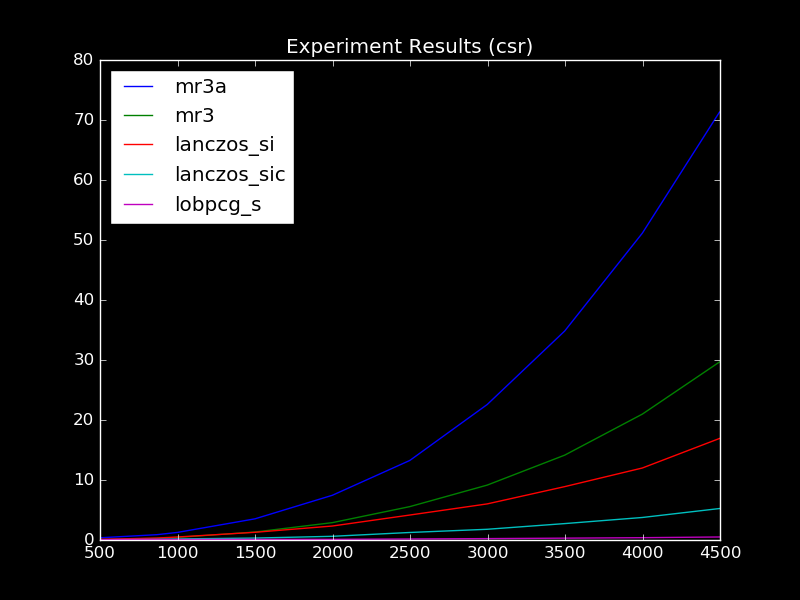
\includegraphics[width=11cm,height=8cm]{results-csr}
\end{figure}

Let us review each line in more detail (we talk mainly about the times
for the biggest matrix):

\begin{itemize}
\item The green line (label \emph{mr3a}) represents the times for the
  MRRR algorithm, for 
  for computing all the eigenpairs. This is not exactly the same time
  the application will get today, as the algorithm is different; but
  it could be considered as a lower bound (given that MRRR is the
  state of the art for dense matrices). We can see that the time for
  the biggest matrix goes a bit higher than 70 seconds.
\item The blue line (label \emph{mr3}) is the MRRR algorithm, but
  taking advantage of its main feature: the ability to compute in
  isolation just the eigenpair we need. We can see that doing so,
  reduces the time to a bit less than 30 secods (for the biggest
  matrix).
\item The orange line (label \emph{lanzos\_si}) is the first sparse
  matrix algorithm; it consists in the Lanczos variant using SuperLU
  as the linear solver. Even when such solver is not specialized for
  the Laplacian matrix, it can reduce the time to 17 seconds
  approximately.
  \item The sky blue line (label \emph{lanzos\_sic}) is the very same
    Lanczos variant, but this time using the Cholmod linear solver. We
    can see that using a more specialized solver, that is optimized
    for Symmetric Positide Definite matrices, pays off; to biggest
    time does down to 5 seconds, approximately.
  \item The Lanczos variant (IRLM), combined with Cholmod linear
    solver, was going to be our best time; until we discovered how to
    avoid the exceptions that the LOBPCG implementation was raising on
    the presence of clustered eigenvalues. That brought this purple
    line (label \emph{lobpcg}), which by far beats them all; the time
    goes into subsecond scale even for the biggest matrix (the actual
    average time is around half a seconf!). This makes LOBPCG the
    definite winner of the experiment. 
    experiment. 
\end{itemize}

The CSC results are basically the same, except for a sharp increment of 300
seconds for the $mr3a$ line (MRRR algorithm against biggest matrix):

\begin{figure}[H]
  \centering
  \includegraphics[width=11cm,height=8cm]{results-csc}
\end{figure}

We can perceive though, that the rest of the lines behave quite the
same, as the following graph shows:

\begin{figure}[H]
  \centering
  \includegraphics[width=11cm,height=8cm]{results-csc-wa}
\end{figure}

Then, using the CSR format should not be considered an advantage for
the algorithms; as the total speedup is actually higher for CSC
format. But again, given the need to run the SCC algorithm, we prefer
CSR.

